\chapter{Elementi caratterizzanti del progetto}
\label{cap:elementi-progetto}
% Qui introdurrò brevemente il contenuto delle sezioni sottostanti.
Questo capitolo si occupa di introdurre gli strumenti utilizzati nel corso del tirocinio, definire e dare una visione concreta delle attività di sviluppo del progetto di \textit{stage} e dare prova dei risultati raggiunti 
a livello di documentazione, di codice scritto, \textit{test coverage} e obiettivi raggiunti. 

\section{Stile lavorativo}

% In questa sezione descriverò il modo in cui ho lavorato nel corso del tirocinio, descrivendo attività esterne allo sviluppo, alla verifica ed alla validazione e descrivendo il modo in cui invece tali attività sono state ideate.
Data la pianificazione a cadenza settimanale delle attività (sezione \hyperref[sec:pianificazione]{§2.5}), ho concordato con il tutor aziendale, il signor \textit{Michele Rigo}, l'organizzazione di una riunione di allineamento settimanale, programmata per ogni lunedì mattina. \\
Tale incontro mirava a:
\begin{itemize}
    \item Mostrare il lavoro svolto nel corso della settimana precedente alla riunione;
    \item Condurre una retrospettiva sulla settimana precedente;
    \item Valutare lo stato di avanzamento del progetto in relazione alle aspettative;
    \item Delineare le attività da svolgere nella settimana in corso.
\end{itemize}

\begin{figure}[H]
    \centering
    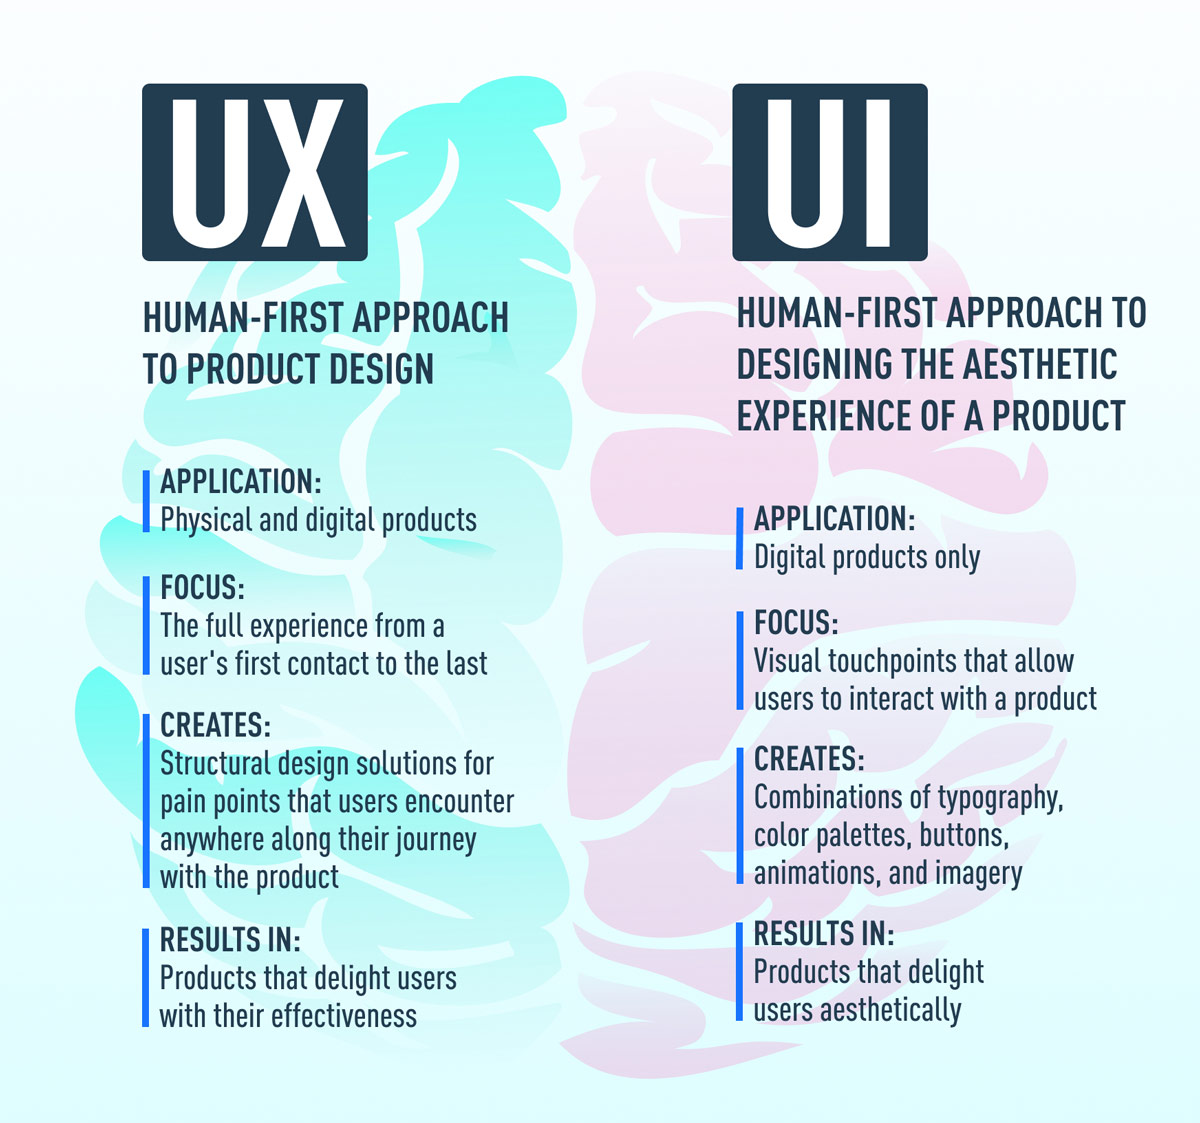
\includegraphics[width=0.7\textwidth]{images/difference-between-ux-and-ui.jpg}
    \caption[Confronto tra la progettazione di interfacce e di esperienze utente]{Confronto tra la progettazione di interfacce (\textit{UI}) e di esperienze utente (\textit{UX})\footnotemark}
\end{figure}
\footnotetext{Fonte: \href{https://careerfoundry.com/en/blog/ux-design/the-difference-between-ux-and-ui-design-a-laymans-guide/}{https://careerfoundry.com}}
Abbiamo svolto degli incontri aggiuntivi in forma telematica per chiarire alcuni aspetti del progetto, in particolare la comprensione di alcuni requisiti utente e la definizione di determinati aspetti 
di interfaccia grafica ed esperienza utente (ovvero come l'utente può interagire con l'interfaccia grafica, la relazione che intercorre tra essi). \\
Per tutta la durata delle attività di \textit{stage}, sono stato affiancato in caso di necessità da praticamente tutto il \textit{team \textbf{Trizeta}}, soprattutto per quanto concerne la progettazione dell'interfaccia grafica.

\section{Strumenti utilizzati}

In questa sezione descriverò gli strumenti utilizzati nel corso del progetto, suddividendoli in base alle attività in cui essi sono stati impiegati.

\section{Analisi dei requisiti utente}

In questa sezione descriverò lo scopo dell'analisi dei requisiti in un progetto, le problematiche riscontrate e mostrerò i principali casi d'uso ed i principali requisiti elaborati.

\section{Progettazione}

In questa sezione descriverò lo scopo della progettazione in un progetto, le problematiche riscontrate e mostrerò le classi (e le loro dipendenze, quando utile e possibile, tramite il linguaggio UML) relative ai principali requisiti analizzati nella sezione precedente in modo da dare riscontro effettivo del passaggio da "requisito" a "scelta progettuale".
In questa sezione includerò anche la progettazione dell'interfaccia grafica relativa alle classi sopra indicate.

\section{Codifica}

In questa sezione descriverò lo scopo della codifica in un progetto ed indicherò le problematiche riscontrate.

\section{Verifica}

In questa sezione descriverò le modalità con le quali si è accertato che l’esecuzione delle attività (per un determinato periodo di tempo) non abbia introdotto errori.

\section{Validazione}

In questa sezione descriverò le modalità con le quali si è accertato che il prodotto finito fosse conforme alle aspettative.

\section{Statistiche qualitative e quantitative finali}

In questa sezione descriverò i prodotti di progetto dal punto di vista della qualità (qui vi sarà particolare enfasi sul prodotto software) e della quantità.